\documentclass{beamer}
\usepackage{../tut-slides}
\usepackage{../mathoperatorsAuD}

\usepackage{amsmath,amssymb}
\usepackage{stmaryrd}
\usepackage{enumerate}
%\usepackage[inline]{enumitem} 		%customize label
%\newcommand{\labelitemi}{\raisebox{1pt}{\scalebox{.9}{$\blacktriangleright$}}}
%\newcommand{\labelitemii}{$\vartriangleright$}
%\newcommand{\labelitemiii}{--}
\setbeamertemplate{itemize item}{\raisebox{1pt}{\scalebox{.9}{$\blacktriangleright$}}}
\setbeamertemplate{itemize subitem}{$\vartriangleright$}

\usepackage{booktabs}
\usepackage{tabularx}
\usepackage{tabu}
\newcommand*\head{\rowfont{\bfseries}}
\newcommand*{\tw}{\rowfont{\ttfamily}}
\renewcommand{\tabularxcolumn}[1]{>{\hspace{0pt}}m{#1}}

\usepackage{cancel}

\usepackage{empheq}
\newcommand*\widefbox[1]{\fbox{\hspace{2em} #1 \hspace{2em}}}

\usepackage{tcolorbox}
\newtcolorbox{mymathbox}[1][]{colback=white, sharp corners, #1}

%%%% EBNF-Terme %%%%
\newcommand{\wdh}[1]{\hat{\{} \ #1 \ \hat{\}}}
\newcommand{\opt}[2]{\hat{(} \ #1 \ \hat{|} \ #2 \ \hat{)}}
\newcommand{\byp}[1]{\hat{[} \ #1 \ \hat{]}}
\newcommand{\rdb}[1]{\hat{(} \ #1 \ \hat{)}}

\newcommand{\sem}[1]{\left\llbracket #1 \right\rrbracket}


\begin{document}	
	\title{Algorithmen und Datenstrukturen}
	\subtitle{Übung 4: Extended Backus-Naur-Form}
	\author{Eric Kunze}
	\email{eric.kunze@mailbox.tu-dresden.de}
	\city{TU Dresden}
%	\institute{Lehrstuhl für Grundlagen der Programmierung}
	\titlegraphic{\includegraphics[width=2cm]{../TUD-white.pdf}}
	\date{14.11.2019}

	\maketitle


%%%%%%%%%%%%%%%%%%%%%%%%%%%%%%%%%%%%%%%%%%%%%%%%%%%%%%%%%%%%%%%%%%%%%%%%%%%%%

%\begin{frame} \frametitle{EBNF-Definition}
%	\small
%	\begin{itemize}
%		\item EBNF-Definition besteht aus endlicher Menge von EBNF-Regeln.
%		\item Jede EBNF-Regel besteht aus einer linken und einer rechten Seite, die rechte Seite ist ein EBNF-Term.
%	\end{itemize}
%	\pause
%	\begin{block}{Definition: EBNF-Term}
%		Seien $V$ eine endliche Menge (syntaktische Variablen) und $\Sigma$ eine endliche Menge (Terminalsymbole) mit $V \cap \Sigma = \emptyset$. Die Menge der EBNF-Terme über $V$ und $\Sigma$ (notiere: $T(\Sigma, V)$), ist die kleinste Menge $T \subseteq \brackets{V \cup \Sigma \cup \menge{\hat{\{}, \hat{\}}, \hat{[}, \hat{]}, \hat{(}, \hat{)}, \hat{|}}}$ mit $V \subseteq T$, $\Sigma \subseteq T$ und
%		\begin{itemize}
%			\item Wenn $\alpha \in T$, so auch $\rdb{\alpha} \in T$, $\wdh{\alpha} \in T$, $\byp{\alpha} \in T$.
%			\item Wenn $\alpha_1, \alpha_2 \in T$, so auch $\opt{\alpha_1}{\alpha_2} \in T$, $\alpha_1 \alpha_2 \in T$
%		\end{itemize}
%	\end{block}
%\end{frame}

\begin{frame} \frametitle{Übersetzung Syntaxdiagramme $\leftrightarrow$ EBNF}
	\centering
	\includegraphics[width=.9\textwidth]{tut04_trans.jpg}
\end{frame}

\begin{frame} \frametitle{Semantik von EBNF-Termen}
	\begin{itemize}
		\item Sei $\mathcal{E} = (V,\Sigma,S,R)$ eine EBNF-Definition.
		\item $v \in V \leadsto W(\mathcal{E},v) = \rho(v)$ (syntaktische Kategorie)
		\item Semantik $\abb{\sem{\cdot}}{\underbrace{T(\Sigma, V)}_{\alpha}}{((\underbrace{V \to \pows{\Sigma^\ast}}_{\rho}) \to \pows{\Sigma^\ast})}$
		\item[] \includegraphics[width=.9\textwidth]{tut04_semantik.jpg}
	\end{itemize}	
\end{frame}

\section{Übungsblatt 3}

\begin{frame} \frametitle{Aufgabe 4 --- Teil (a)}
	$W(\mathcal{E},S) = \menge{a^{n+m} w b^\ell a^n \mid n,m \ge 0, 0 \le \ell \le m, w \in \Sigma^\ast}$
	\pause
	\begin{align*}
	V = \menge{S,A,B} \quad \und \quad  
	R = \Big\{ S &::= \opt{aSa}{A} ,\\
	A & ::= \opt{aA \byp{b}}{B}, \\
	B & ::= \wdh{\opt{a}{b}} \quad \Big\}
	\end{align*}
\end{frame}

\begin{frame} \frametitle{Aufgabe 4 --- Teil (b)}
	\begin{align*}
		f(\rho) = \begin{pmatrix} f(\rho)(S) \\ f(\rho)(A) \end{pmatrix} 
		= \begin{pmatrix} \sem{\byp{aAb}}(\rho) \\ \sem{\opt{Sc}{cS}}(\rho) \end{pmatrix} 
		= \begin{pmatrix}
		\menge{a} * \rho(A) * \menge{b} \\ \rho(S) * \menge{c} \cup \menge{c} * \rho(S)
		\end{pmatrix}
	\end{align*}
	\pause
	\begin{align*}
		\begin{pmatrix} \emptyset \\ \emptyset \end{pmatrix}
		\overset{f}{\mapsto}
		\begin{pmatrix} \menge{\epsilon} \\ \emptyset \end{pmatrix}
		\overset{f}{\mapsto}
		\begin{pmatrix} \menge{\epsilon} \\ \menge{c} \end{pmatrix}
		\overset{f}&{\mapsto}
		\begin{pmatrix} \menge{\epsilon,acb} \\ \menge{c} \end{pmatrix} \\
		\overset{f}&{\mapsto}
		\begin{pmatrix} \menge{\epsilon,acb} \\ \menge{c,acbc,cacb} \end{pmatrix} \\
		\overset{f}&{\mapsto}
		\begin{pmatrix} \menge{\epsilon,acb,aacbcb,acacbb} \\ \menge{c,acbc,cacb} \end{pmatrix}
	\end{align*}
\end{frame}

\begin{frame} \frametitle{Aufgabe 4 --- Teil (c)}
	\centering
	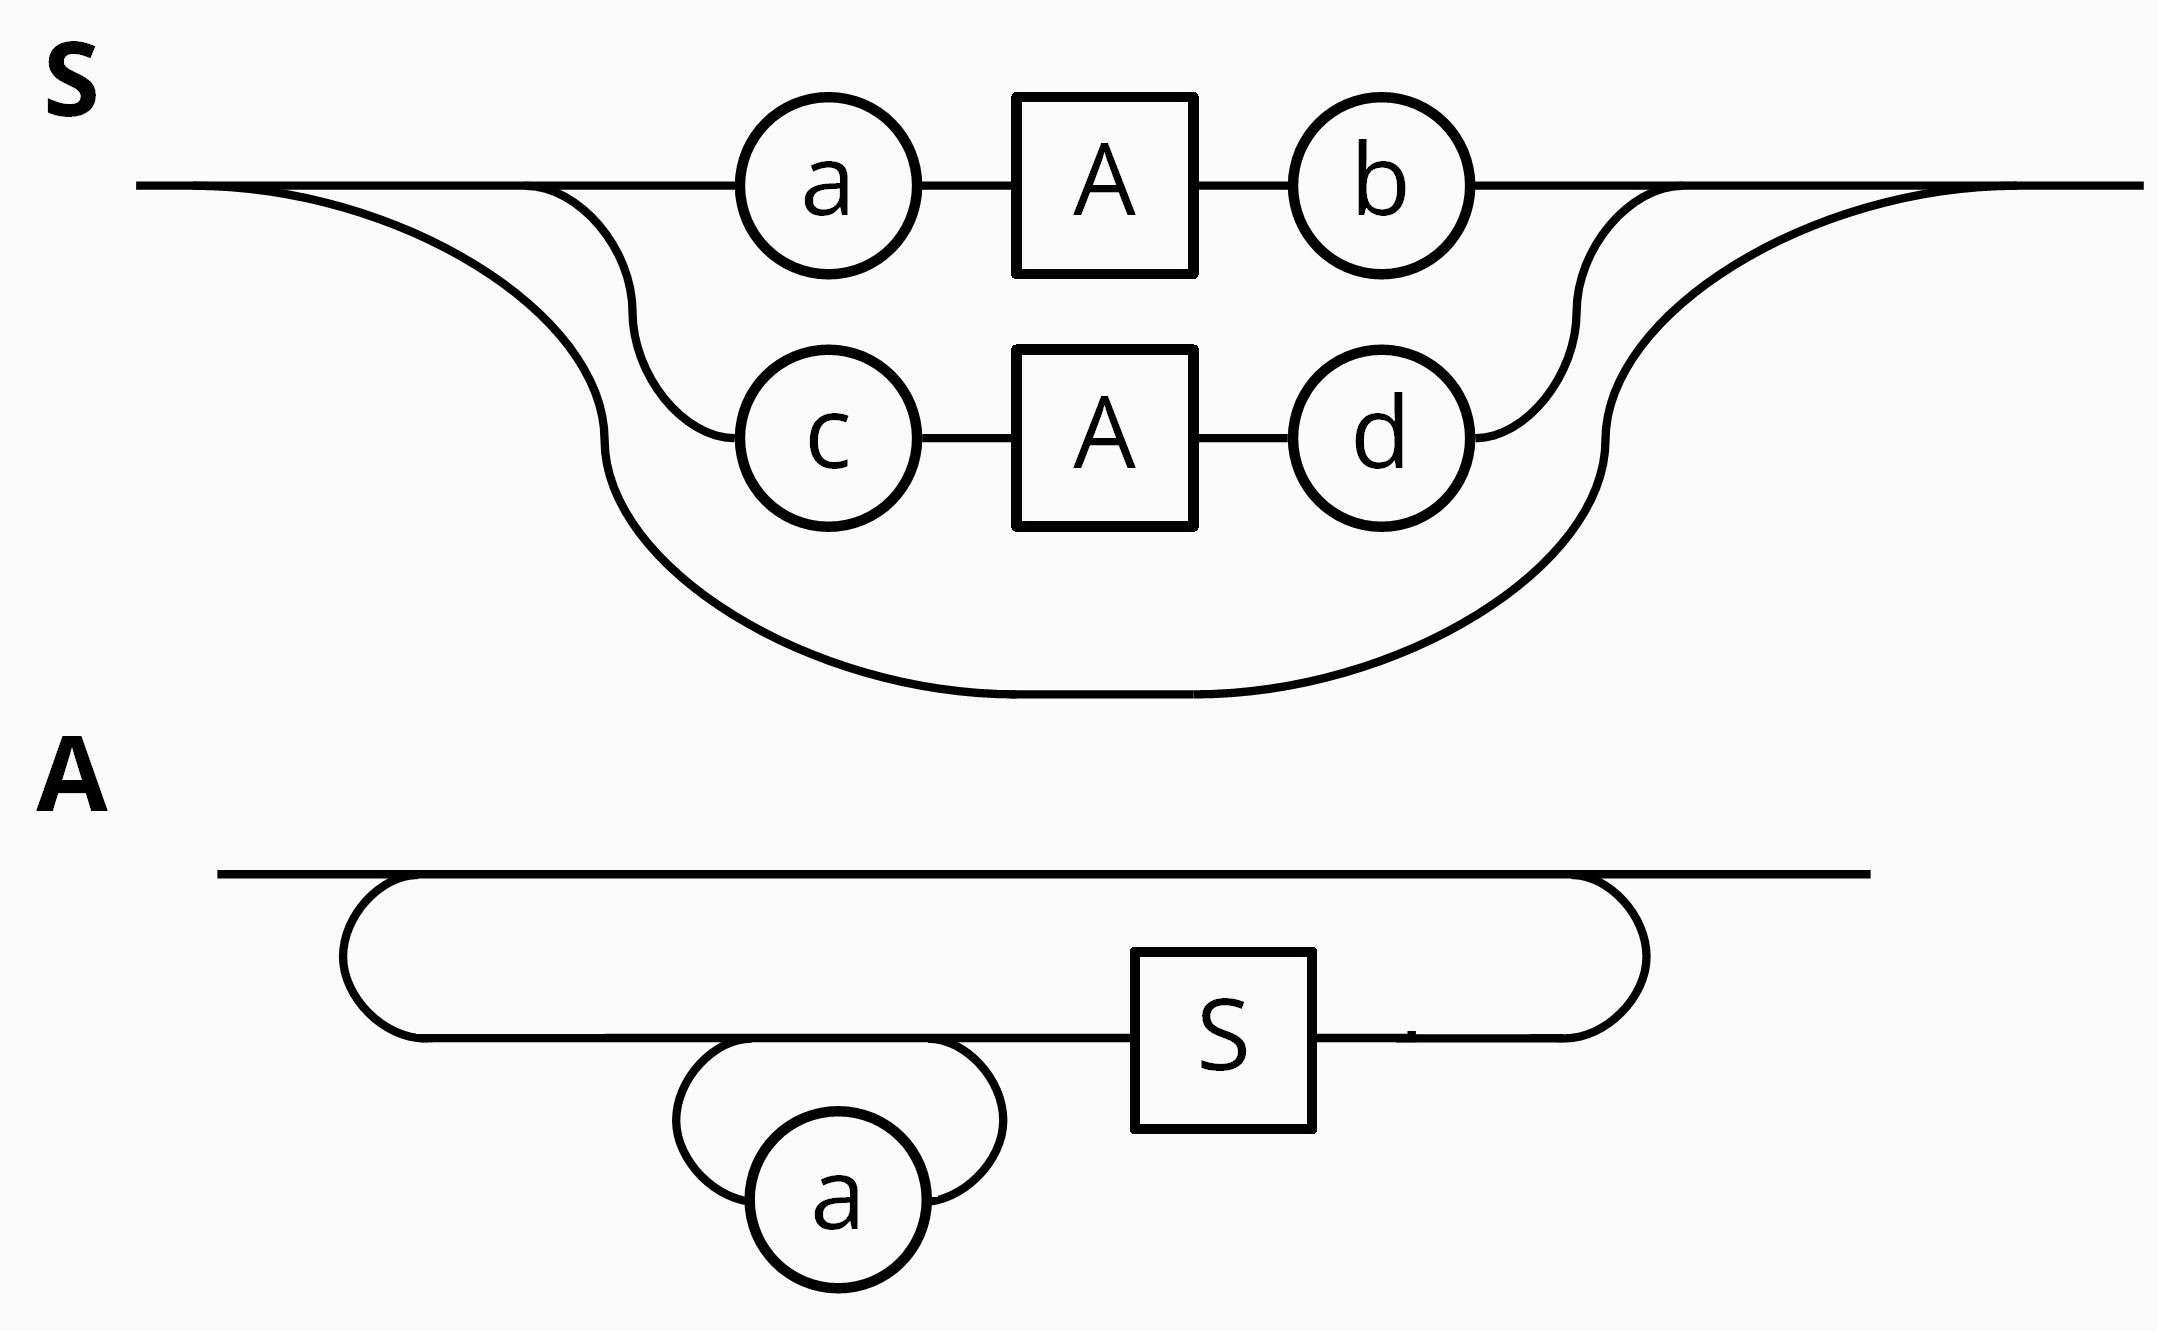
\includegraphics[width=\textwidth]{tut03_syntax_dia_4c.jpg}
\end{frame}

\section{Übungsblatt 4}

\begin{frame} \frametitle{Aufgabe 1 --- Teil (a)}
	\begin{align*}
		f(\rho) = \begin{pmatrix} f(\rho)(S) \\ f(\rho)(B) \end{pmatrix} 
		= \begin{pmatrix} \sem{\byp{B} \ b}(\rho) \\ \sem{Sb}(\rho) \end{pmatrix} 
		&= \begin{pmatrix}
		\brackets{\rho(B) \cup \menge{\epsilon}} * \menge{b} \\ \rho(S) * \menge{b}		\end{pmatrix} \\
		&= \begin{pmatrix}
		\rho(B) * \menge{b} \cup \menge{b} \\ \rho(S) * \menge{b}		\end{pmatrix}
	\end{align*}
	\pause
	\hrule
	Fünf Iterationen:
	\begin{align*}
		\begin{pmatrix} \emptyset \\ \emptyset \end{pmatrix}
		\overset{f}{\mapsto}
		\begin{pmatrix} \menge{b} \\ \emptyset \end{pmatrix}
		\overset{f}{\mapsto}
		\begin{pmatrix} \menge{b} \\ \menge{b^2} \end{pmatrix}
		\overset{f}{\mapsto}
		\begin{pmatrix} \menge{b,b^3} \\ \menge{b^2} \end{pmatrix} 
		\overset{f}&{\mapsto}
		\begin{pmatrix} \menge{b,b^3} \\ \menge{b^2,b^4} \end{pmatrix}  \\
		\overset{f}&{\mapsto}
		\begin{pmatrix} \menge{b,b^3,b^5} \\ \menge{b^2,b^4} \end{pmatrix}
	\end{align*}
\end{frame}

\begin{frame} \frametitle{Aufgabe 1 --- Teil (b)}
	\begin{align*}
		\dots \overset{f}{\mapsto}
		\begin{pmatrix} \menge{b,b^3,b^5} \\ \menge{b^2,b^4} \end{pmatrix}
	\end{align*}
	
	\pause
	
	\begin{align*}
	\implies W(\mathcal{E},S) &= \menge{b^{2n+1} \mid n \ge 0}  \\
	W(\mathcal{E},B) &= \menge{b^{2n+2} \mid n \ge 0} = \menge{b^{2n} \mid n \ge 1}
	\end{align*}
\end{frame}

\begin{frame} \frametitle{Aufgabe 1 --- Teil (c)}
	\small 
	Vermutung: 
	\begin{align*}
		W(\mathcal{E},S) = \menge{b^{2n+1} \mid n \ge 0}  \quad \und \quad
		W(\mathcal{E},B) = \menge{b^{2n} \mid n \ge 1}
	\end{align*}
	
	\pause
%	\footnotesize
		
	\begin{align*}
	  \sem{S}(\rho) & = \sem{\byp{B} \ b}(\rho) & 											\sem{B}(\rho) & = \sem{S \ b}(\rho) \\
					& = \brackets{\sem{B}(\rho) \cup \menge{\epsilon}} * \sem{b}(\rho) &			      & = \sem{S}(\rho) * \sem{b}(\rho) \\
					& = \brackets{\rho(B) \cup \menge{\epsilon}} * \menge{b} &							  & = \rho(S) * \menge{b} \\
					& = \rho(B) * \menge{b} \cup \menge{b} &											  & = \menge{b^{2n+1} \mid n \ge 0} * \menge{b} \\ 			
					& = \menge{b^{2n} \mid n \ge 1} * \menge{b} \cup \menge{b} &						  & = \menge{b^{2n+2} \mid n \ge 0} \\	
					& = \menge{b^{2n+1} \mid n \ge 1} \cup \menge{b^{2*0+1}} & 						      & = \menge{b^{2n} \mid n \ge 1} \\
					& = \menge{b^{2n+1} \mid n \ge 0} &													  & = W(\mathcal{E},B) \\
					& = W(\mathcal{E},S)
	\end{align*}
\end{frame}

\begin{frame} \frametitle{Aufgabe 2 --- Teil (a)}
	\centering
	\includegraphics[width=\textwidth]{tut04_syntax_dia_2a.jpg}
\end{frame}

\begin{frame} \frametitle{Aufgabe 2 --- Teil (b)}
	\small
	\begin{align*}
		f(\rho) = \begin{pmatrix} f(\rho)(S) \\ f(\rho)(A) \\ f(\rho)(B) \end{pmatrix} 
		&= \begin{pmatrix} \sem{AB}(\rho) \\ \sem{\opt{aAc}{\wdh{b}}}(\rho) \\ \sem{d \ \byp{B} \ c}(\rho) \end{pmatrix} \\
		&= \begin{pmatrix}
			\rho(A) * \rho(B) \\ \menge{a} * \rho(A) * \menge{c} \cup \menge{b}^\ast \\ \menge{d} * \brackets{\rho(B) \cup \menge{\epsilon}} * \menge{c} \end{pmatrix} \\
		&= \begin{pmatrix}
			\rho(A) * \rho(B) \\ \menge{a} * \rho(A) * \menge{c} \cup \menge{b}^\ast \\ \menge{d} * \rho(B) * \menge{c} \cup \menge{dc} \end{pmatrix}
	\end{align*}
	
	\begin{align*}
		\begin{pmatrix} \emptyset \\ \emptyset \\ \emptyset \end{pmatrix}
		\overset{f}{\mapsto}
		\begin{pmatrix} \emptyset \\ \menge{b}^\ast \\ \menge{dc} \end{pmatrix}
		\overset{f}{\mapsto}
		\begin{pmatrix} \menge{b^m dc \mid m \in \N} \\ \menge{a^\ell b^m c^\ell \mid \ell \in \menge{0,1}, m \in \N} \\ \menge{d^n c^n \mid n \in \menge{1,2}} \end{pmatrix}
	\end{align*}
\end{frame}

\begin{frame} \frametitle{Aufgabe 2 --- Teil (c)}
	Wir wollen eine EBNF-Definition $\mathcal{E}' = (V,\Sigma,S,R)$ finden, sodass 
	\begin{align*}
		W(\mathcal{E}') &= \menge{a^{n+\ell} c b^n (cd)^\ell \mid n, \ell \in \N, n \ge 1}
		%
		\intertext{gilt. Wir zerlegen wie üblich die Sprache in unabhängige Teile:}
		%
		L &= \menge{\textcolor{cdpurple}{a^\ell} \enskip \textcolor{cdorange}{a^n} \ c \ \textcolor{cdorange}{b^n} \enskip \textcolor{cdpurple}{(cd)^\ell} \mid n,\ell \in \N, n \ge 1}
		%
		\intertext{Dann ergibt sich also nach dem Grundschema}
		%
		V &= \menge{S,A} \\
		R &= \menge{S ::= \opt{aScd}{A} , A ::= \opt{aAb}{acb}}
	\end{align*}
\end{frame}

\end{document}